\subsection{Administrationssystem}
I de følgende afsnit vild er kunne læses om unittests for Administrationssystemet.\\\\


\textbf{Introduktion}\\
Administrationssystemet har været testet itterativt over udviklingsperioden. Det har bidgraget væsentligt med at finde små fejl, som ellers var gået igennem. I de nedenstående afsnit vil der kunne læses om hvordan der er testet, med hvilke frameworks og mere konkrete tal.\\



\textbf{Testdetaljer}\\
I administrationssystemet er der en total testcoverage på \textit{72 procent} af testbare klasser\footnote{GUI, eksterne klasser, XML mv er \textit{ikke} en del af testbare klasser.}. Dette summerer sig op til \textit{111} unittests, som er fordelt over viewmodels og models\footnote{Se eventuelt oversigtsdiagram på figur \ref{fig:oversigtAs}, side \pageref{fig:oversigtAs}}. 

	\begin{figure}[H]
		\centering
		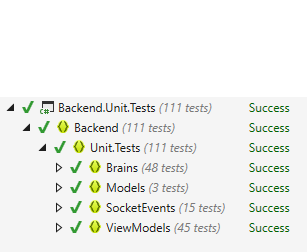
\includegraphics[width=0.50\textwidth]{Test/Images/Backend/AntalUnit.png}
		\caption{Antal unittests for Administrationssystem}
		\label{fig:antalunit}
	\end{figure}

\begin{figure}[H]
	\centering
	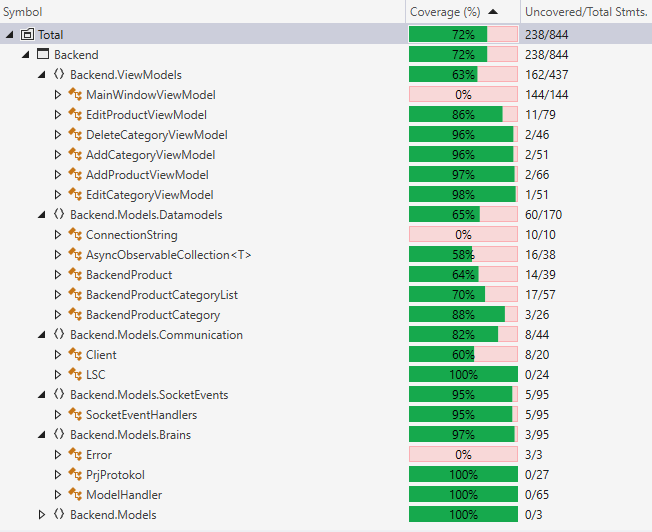
\includegraphics[width=0.90\textwidth]{Test/Images/Backend/Coverage.png}
	\caption{Testcoverage for Administrationssystem}
	\label{fig:cover}
	\end{figure}
	

	
\textbf{Beskrivelse af tests}\\
I \gls{AS}et har der været stor fokus på at teste ModelHandleren\footnote{ModelHandleren ses på figur \ref{fig:modelhandlerreal} på side \pageref{fig:modelhandlerreal}}, da denne har stort ansvar i form af at håndtere data der skal sendes ud. Samtidig har der været en del tests ved SocketEventHandlers\footnote{SocketEventHandlers ses på figur \ref{fig:SocketEventHandlers} side \pageref{fig:SocketEventHandlers}}, da det er dem der har ansvaret for at behandle modtaget data. Dog har det været besluttet at undlade at tage views, properties, XAML og lignende klasser ud af testcoverage, da disse ikke har været testbare og/eller er eksterne biblioteker.\\
 Ligeledes gælder sig for datamodeller, da disse udelukkende arver fra \gls{SL}'s modeller, og kun implementerer INotifyProperyChanged som forskel. \\
 \\
 Der er, som det kan ses i figur \ref{fig:cover}, enkelte dele af systemet som ikke har været testbart. Det gør sig dældende for bl.a. grænseflader så som ErrorPrinteren\footnote{Errorprinteren ses på figur \ref{fig:error} side \pageref{fig:error}}. Dette skyldes at det ikke er muligt at teste, at en beskedboks vises, dog kan der testes at selve printeren bliver kaldt. Dette gør sig også gældende for de andre grænseklasser som findes i systemet - der testes at de modtager.